\section{Contextual Bandit: LinUCB}
We introduced the context-free algorithm in detail last semester, so we will not continue to elaborate on it in this report. Instead, we will focus on the contextual bandit, implementing and verifying one of the most famous algorithms – LinUCB which was proposed by the authors in \cite{context}. LinUCB is an extension of the UCB algorithm. The algorithm chooses an arm based on observation of the current user and set of arms together with the context feature.  Also, in the LinUCB algorithm, there exists a factor $\alpha$, which is used to control the trade-off between exploration and exploitation.

\begin{figure}[htbp]
\centering
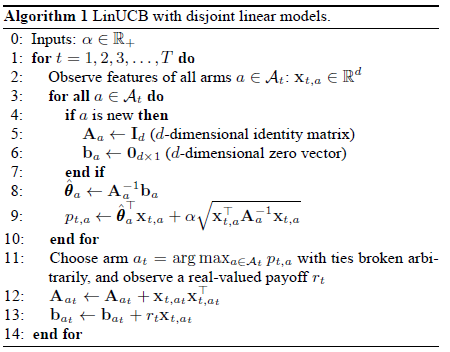
\includegraphics[scale=0.8]{figure/alg1.png}
\caption{LinUCB with disjoint linear models \cite{context}}
\end{figure}

\begin{figure}[htbp]
    \centering
    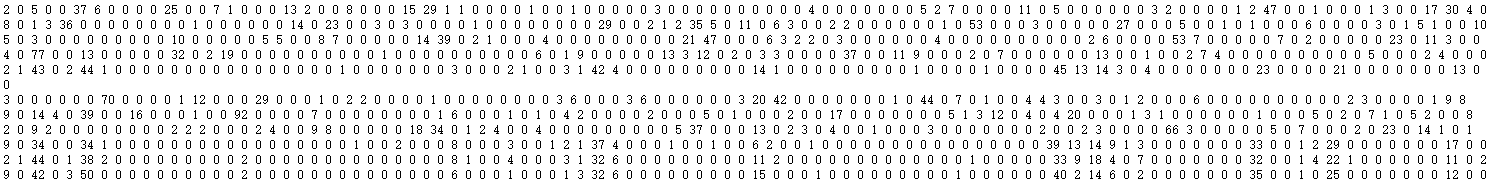
\includegraphics[scale =0.4]{figure/data1.png}
    \caption{Format of the personalization dataset}
    \end{figure}
\textbf{\textit{Dataset}}. For this experiment, the personalization dataset\footnote[3]{Dataset from: http://www.cs.columbia.edu/~jebara/6998/dataset.txt} has been used. Figure 4.2 demonstrates the format of the dataset. This dataset consists of a matrix of size $10000 \times 102$. The data in the first column indicates the action has been chosen. The second column is value indicate the obtained reward, where $y_{t}$ denote the real reward that was obtained at time $t$ and $y_{t}\in \mathbb{B}$. From column 3 to column 103 are the context which is represented as the feature vector $\mathbf{x_{t}}\in\mathbb{R}^{100}$.

\textbf{\textit{Compute click-through rate (CTR)}}. The click-through rate (CTR) proposed in \cite{ctr} is used to evaluate the performance of the algorithm. The click-through rate replay at time $T$ is:
    \begin{equation}
        C(T)=\frac{\sum_{t=1}^{T} y_{t} \times \mathbf{1}\left[\pi_{t-1}\left(\mathbf{x}_{t}\right)=a_{t}\right]}{\sum_{t=1}^{T} \mathbf{1}\left[\pi_{t-1}\left(\mathbf{x}_{t}\right)=a_{t}\right]}
    \end{equation}
where, $\pi_{t-1}$ denote the algorithm trained on data up to time $t-1$. At time $t$, if the context $\mathbf{x}_{t}$ been observed by algorithm $\pi_{t-1}$, then we use the notation $\pi_{t-1}(\mathbf{x}_{t})$ denote the chosen action. $a_{t}$ and $y_{t}$ denote the real action that was taken in the dataset at time $t$ and the real reward that was obtained at time $t$ respectively.

\textbf{\textit{Experiment}}. In this experiment (ideas and parameters are referenced from \cite{experiment}), the size of the context is 100, where $\mathbf{x_{t}}\in \mathbb{R}^{100}$, the number of arms $K=10$, total iteration $T=10000$. For the $\alpha$, as the only input in the algorithm, optimizing this parameter may result in higher total payoffs in practice. So, we will experiment with the blow values of $\alpha$:
\begin{enumerate}
   
    \item For Alpha = 1
     \item For Alpha = 0.25
    \item For Alpha = ${1}/{\sqrt{t}}$
    \item For Alpha = 0.001
    \item For Alpha = $0.001/(0.1 * Prediction Count)$
    
\end{enumerate}
\begin{figure}[htbp]
    \centering
    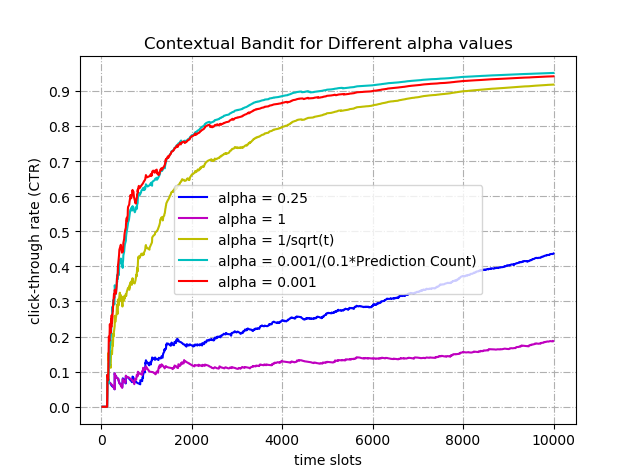
\includegraphics[scale =0.7]{figure/F5.png}
    \caption{CTR of LinUCB for varying Alphas}
    \end{figure}
The click-through rate (CTR) proposed in A is used to evaluate the performance of the algorithm. As it is evident from Figure 4.3, the best CTR value was achieved with an alpha equal to $0.001/(0.1 * Prediction Count)$ when the CTR value was 0.95, where the prediction count is the number of correct predictions.

To understand the trade-off between exploration and exploitation, for each alpha value, first the mean value of the upper confidence bound for 10 arms will be plotted. We will then compare the number of predictions made by each arm with the number of true predictions it made.
\begin{frame}{}
\begin{figure}[htbp]
\centering
\subfigure[MeanUCB]{
\begin{minipage}[t]{0.5\linewidth}
\centering
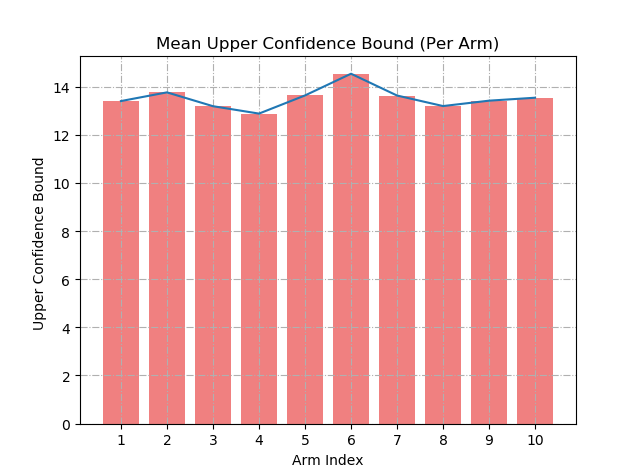
\includegraphics[scale=0.5]{figure/F2.png}
%\caption{fig1}
\end{minipage}%
}%
\subfigure[Prediction comparison]{
\begin{minipage}[t]{0.5\linewidth}
\centering
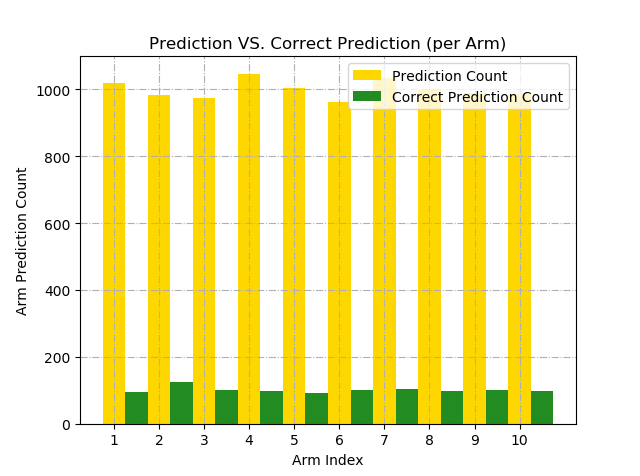
\includegraphics[scale=0.5]{figure/F2.1.png}
%\caption{fig2}
\end{minipage}%
}%
\centering
\caption{ Mean UCB and Total VS. Correct prediction for
Alpha = 1}
\end{figure}  
\end{frame}

As it is evident from Figure 4.4, when the $\alpha$ value is 1, the exploration and exploitation here is at a minimum, which can be represented by strips of nearly the same length. That implies that the upper confidence bound of each arm is very approximate. For this cause, we can also observe that the predicted counts are nearly the same for all arms,thus when the $\alpha$ value equals to 1, the algorithm giving the lowest click rate value which is 0.18 as shown in Figure 4.3.
\begin{figure}[htbp]
\centering
\subfigure[MeanUCB]{
\begin{minipage}[t]{0.5\linewidth}
\centering
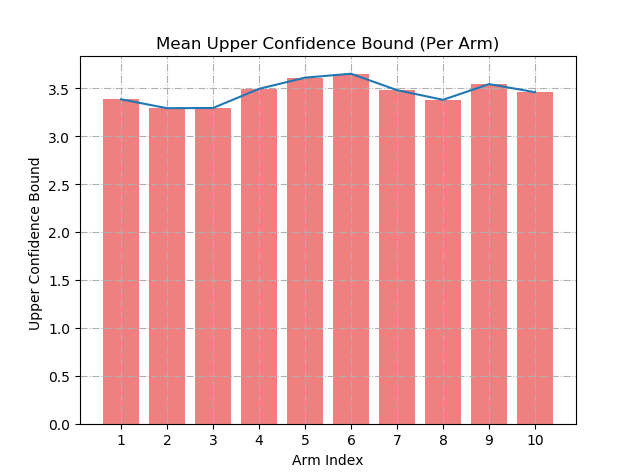
\includegraphics[scale=0.5]{figure/f0.25.png}
%\caption{fig1}
\end{minipage}%
}%
\subfigure[Prediction comparison]{
\begin{minipage}[t]{0.5\linewidth}
\centering
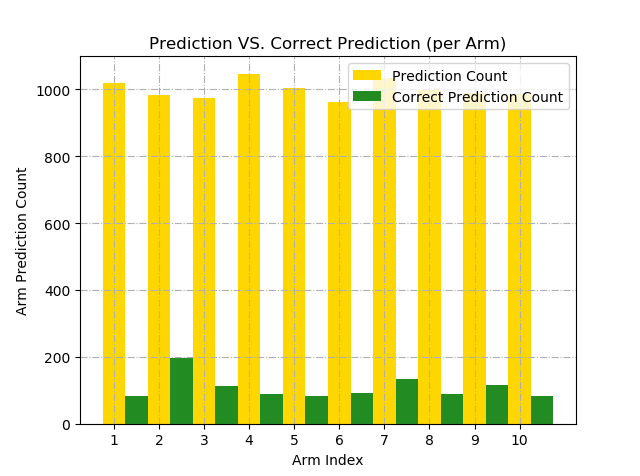
\includegraphics[scale=0.5]{figure/f0.25.2.png}
%\caption{fig2}
\end{minipage}%
}%
\centering
\caption{ Mean UCB and Total VS. Correct prediction for
Alpha = 0.25}
\end{figure}  
For Figure 4.5, When the $\alpha$ value change to 0.25, the improvement is not significant compare to the result when $\alpha$ value equals to 1 .
\begin{figure}[htbp]
\centering
\subfigure[MeanUCB]{
\begin{minipage}[t]{0.5\linewidth}
\centering
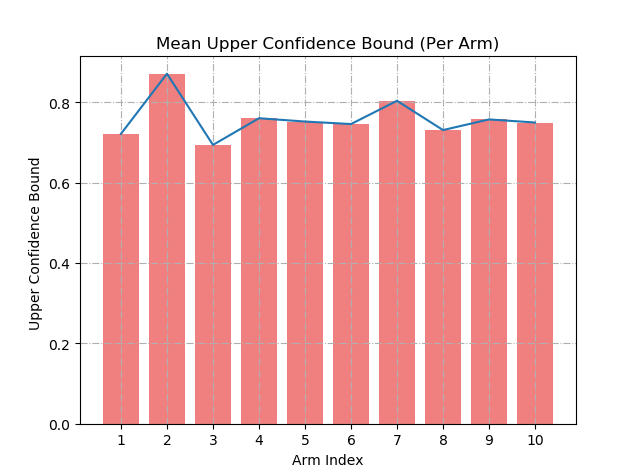
\includegraphics[scale=0.5]{figure/F3.png}
%\caption{fig1}
\end{minipage}%
}%
\subfigure[Prediction comparison]{
\begin{minipage}[t]{0.5\linewidth}
\centering
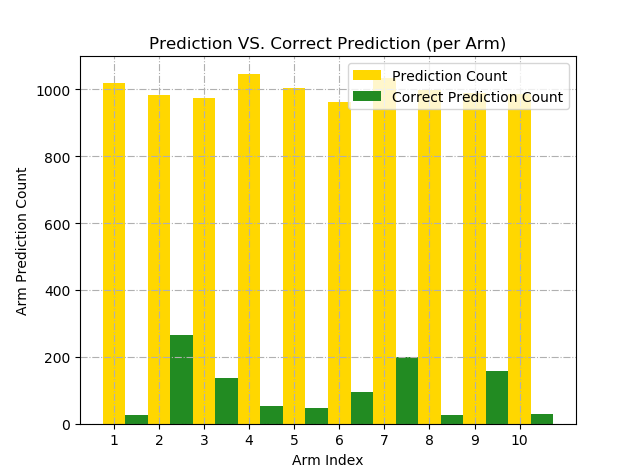
\includegraphics[scale=0.5]{figure/F3.1.png}
%\caption{fig2}
\end{minipage}%
}%
\centering
\caption{ Mean UCB and Total VS. Correct prediction for
Alpha = ${1}/{\sqrt{t}}$}
\end{figure}  
Now, when we change our $\alpha$ to the time-dependent values (i.e., square root of the time), as shown in Figure 4.6, the result receives a significant improvement. This is mainly caused by the fact that we adjust our exploration according to the changes in time and limit our predictions in order to maximize the use of our trained algorithms over time.
\begin{figure}[htbp]
\centering
\subfigure[MeanUCB]{
\begin{minipage}[t]{0.5\linewidth}
\centering
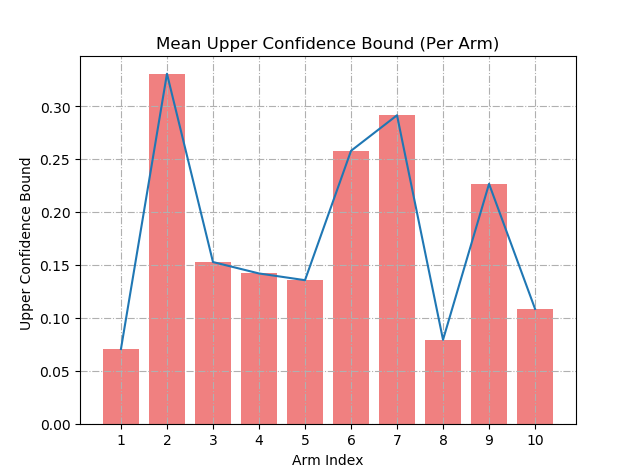
\includegraphics[scale=0.5]{figure/F0.001.png}
%\caption{fig1}
\end{minipage}%
}%
\subfigure[correct prediction comparison]{
\begin{minipage}[t]{0.5\linewidth}
\centering
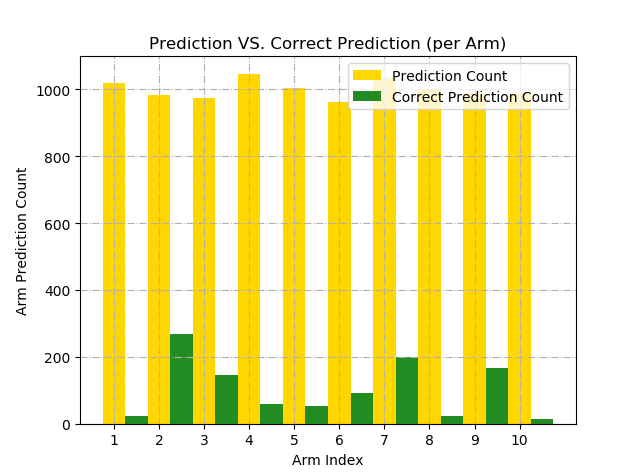
\includegraphics[scale=0.5]{figure/F0.001.2.png}
%\caption{fig2}
\end{minipage}%
}%
\centering
\caption{ Mean UCB and Total VS. Correct prediction for
Alpha = 0.001}
\end{figure}  
Figure 4.7 shows that when $\alpha=0.001$, a higher CTR can get. Because of the extremely small value of $\alpha$, the algorithm will perform exploiting most of the iteration and limiting the exploration.
\begin{figure}[htbp]
\centering
\subfigure[MeanUCB]{
\begin{minipage}[t]{0.5\linewidth}
\centering
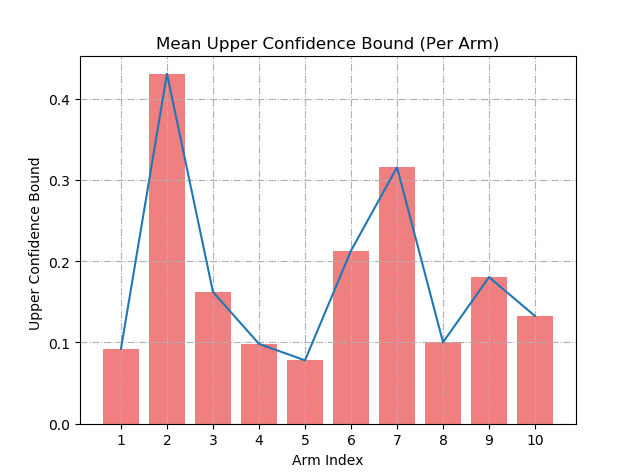
\includegraphics[scale=0.5]{figure/F4.png}
%\caption{fig1}
\end{minipage}%
}%
\subfigure[Prediction comparison]{
\begin{minipage}[t]{0.5\linewidth}
\centering
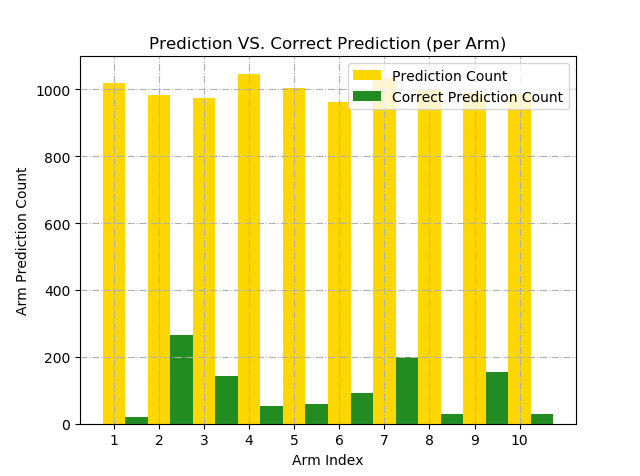
\includegraphics[scale=0.5]{figure/F4.1.png}
%\caption{fig2}
\end{minipage}%
}%
\centering
\caption{ Mean UCB and Total VS. Correct prediction for
Alpha = $0.001/(\frac{correct-predictions}{10})$}
\end{figure}  
In the experiment, we further perform an $\alpha$ value with correct prediction dependent which is the Figure 4.8. The intuition for doing so is that the alpha value related to the correct prediction increases the exploitation of the arm that performs better (i.e., the larger the correct prediction, the smaller the $\alpha$ value). On the other hand, the number of explorations for the arm with inaccurate predictions has increased.

From the above figures, we can see that the arm with the largest upper confidence bound is also the arm with the highest number of predictions. This reflects the nature of the LinUCB algorithm that selects the arm with the highest upper confidence bound as the prediction.
\section{Matrix Factorization Implementation}
To implement the matrix factorization mentioned in section 3.1, a smaller data set was chosen in order for us to carry out a comparison between the two approaches: the base method and the bias method (i.e., the method of matrix factorization that considers both user bias and item bias). 

\textbf{\textit{Dataset}}. The partial dataset is shown in Figure 4.9. The user-item rating matrix $\textit{R}$ is a $25 \times 100$ matrix, which represent 25 users and 100 items. Furthermore, we can see from the figure that  $\textit{R}$ is a sparse matrix (i.e. matrix with many zeros)
\begin{figure}
\centering
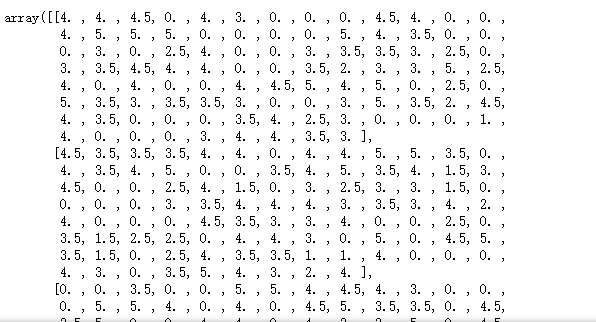
\includegraphics[scale =0.8]{figure/mf1.png}
\caption{Partial  of the user-item rating matrix \textit{R}}
\end{figure}

\textbf{\textit{Training}}.
Recall our loss function:
\begin{equation}
        \text { Loss }: J(p, q)=\min_{ q *, p * } \sum_{(u, i) \in K}\left(r_{u,i}-q_{i}^{T} p_{u}\right)^{2}+\lambda\left(\left\|q_{i}\right\|+\left\|p_{u}\right\|\right)^{2}
\end{equation}
Based on the methods proposed in \cite{mf1}, we use a stochastic gradient descent (SGD) algorithm to train two latent vector matrices: a user latent matrix \textit{p} and item latent matrix \textit{q}.By defining $e_{u,i}=r_{u,i}-q_{i}^{T} p_{u}$. We update the two matrices by the following formulas:
\begin{equation}
    q_{i} \leftarrow q_{i}+\eta\left(e_{u,i} p_{u}-\lambda q_{i}\right)
\end{equation}
\begin{equation}
    p_{u} \leftarrow p_{u}+\eta\left(e_{u,i} q_{i}-\lambda p_{u}\right)
\end{equation}
In the experiment, we set the number of latent features $k=2$, then we initiated the user matrix and item matrix with a size of $25 \times 2$ (i.e., number of users $\times$ number of latent features).
Furthermore, the learn rate$\eta=0.001$, regularization factor$\lambda = 0.1$ and iteration 1000 times.
\begin{figure}[htbp]
\centering
\subfigure[User latent matrix]{
\begin{minipage}[t]{0.5\linewidth}
\centering
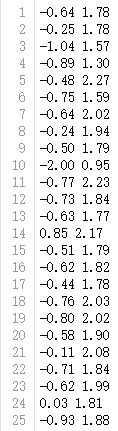
\includegraphics[scale=0.6]{figure/user1.png}
%\caption{fig1}
\end{minipage}%
}%
\subfigure[Item latent matrix (first 25 out of 100 items)]{
\begin{minipage}[t]{0.5\linewidth}
\centering
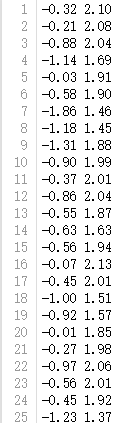
\includegraphics[scale=0.6]{figure/item1.png}
%\caption{fig2}
\end{minipage}%
}%
\centering
\caption{User and item matrix}
\end{figure} 
After iteration, we can get our user latent matrix \textit{p} and item latent matrix \textit{q}, as shown in figure 4.10. Then, by performing the inner product between these two latent matrices, we get the predicted user-item rating matrix $\hat{R}$, shown in Figure 4.11. Expressed by the formula: $\hat{R}$ = user latent matrix $\times$ item latent matrix$^\textbf{T}$.
\begin{figure}[htbp]
\centering
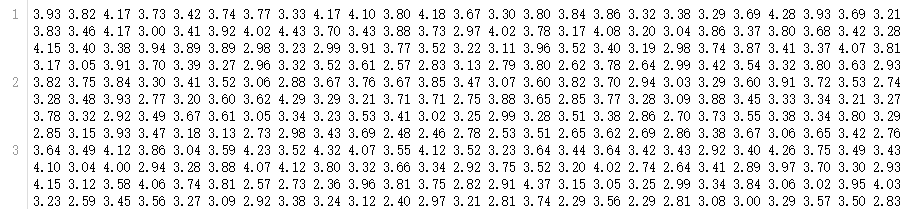
\includegraphics[scale =0.7]{figure/result1.png}
\caption{Predicated rating matrix $\hat{R}$ (Partial,first 3 out of 100 user's estimate rating)}
\end{figure}

\textbf{\textit{Adding bias}}.Now, we will experiment with the bias method, which considers both user bias and item bias. As mentioned before, when we consider the bias, then the loss function becomes:
\begin{equation}
    \operatorname{Loss}=\min _{q^{*}, p^{*}} \sum_{(u, i) \in K}\left(r_{u,i}-b_{u,i}-q_{i}^{T}p_{u}\right)^{2}+\lambda \left(\left\|q_{i}\right\|^{2}+\left\|p_{u}\right\|^{2}+b_{u}^{2}+b_{i}^{2}\right)
\end{equation}
The formula used to iterate over the user latent matrix and the item latent matrix becomes:
\begin{equation}
    q_{i} \leftarrow q_{i}+\eta\left(\left ( r_{u i}-q_{i}^{T} p_{u}-b_{u,i} \right ) p_{u}-\lambda q_{i}\right)
\end{equation}
\begin{equation}
    p_{u} \leftarrow p_{u}+\eta\left(\left ( r_{u i}-q_{i}^{T} p_{u}-b_{u,i} \right ) q_{i}-\lambda p_{u}\right)
\end{equation}
The rest of the steps are consistent with the base matrix factorization method.After the training, we get the user and item latent matrix based on the bias method. By the visualization method, Figure 4.12 plots the latent vectors of users and items in the two-dimensional coordinate. Through multiply the red dot coordinate by the blue cross’s coordinate in the figure, you can get the predicted rating score of user $u$ on item $i$.

\begin{figure}[htbp]
\centering
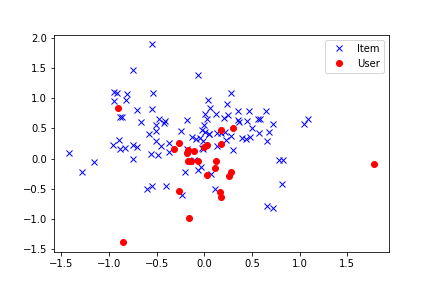
\includegraphics[scale =0.8]{figure/f6.png}
\caption{visualization of user and item latent vector}
\end{figure}

\textbf{\textit{Evaluation}}. To compare the performance between the base method and the bias method, Mean Square Error (MSE) is used to evaluate these two algorithms. In order not to lose generality, we conducted 10 experiments and took the average of the results. What is striking in Table 4.1 is the dramatic decline of MSE, when we consider user bias and item bias, the value of MSE is reduced by $20\%$ which proved that consider both user and item bias when
perform the matrix factorization is effective.


\begin{table}[htbp]
\centering
\begin{tabular}{lll}
\hline
            &\textbf{MSE}    & \textbf{Improvement rate} \\ \hline
Base method  $\hat{r}_{u,i}=q_{i}^{T}p_{u}$ & 0.6530 &                  \\
Bias method $\hat{\boldsymbol{r}}_{u,i}=b_{u,i}+q_{i}^{T} p_{u}$ & 0.5178 & 20.715\%        
\end{tabular}
\caption{Evaluation between base method and bias method}
\end{table}